\section{GridCurve}

\begin{frame}
  \frametitle{GridCurve}

  \begin{block}{What ?}
GridCurve is an (open or closed) $d$-dimensional oriented grid curve 
lying in a $n$-dimensional cellular space. 
It stores a list of (signed) $1$- or $(n-1)$-cells. 
  \end{block}

 \begin{figure}
   \centering
   \subfigure[$d = 1, n = 2$]{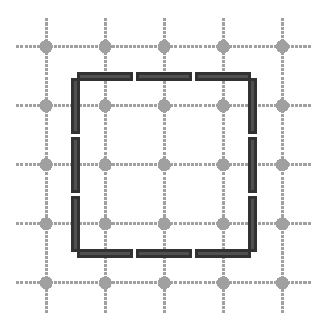
\includegraphics[width=0.25\textwidth]{1cellsRange}}
   \subfigure[$d = 1, n = 3$]{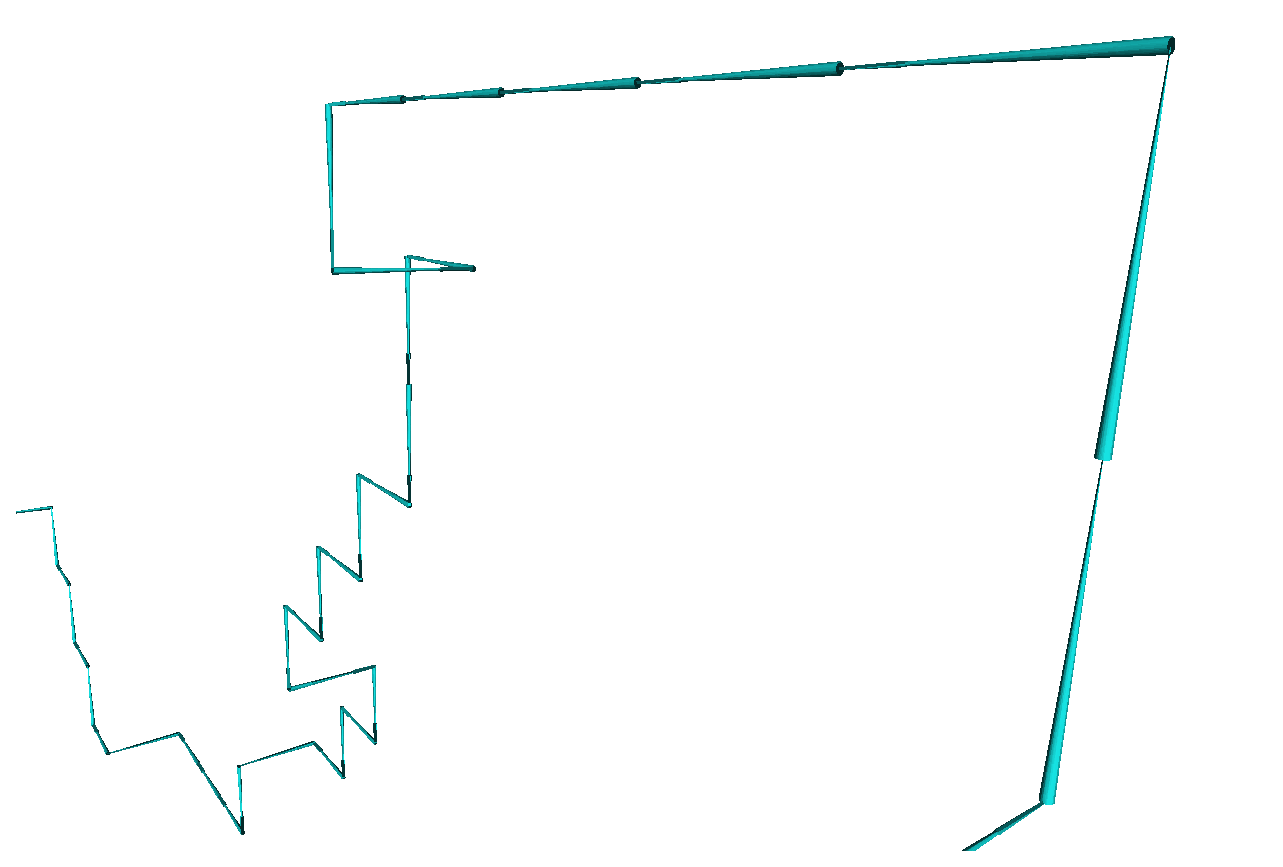
\includegraphics[width=0.35\textwidth]{gridCurve3d1}}
   \subfigure[$d = 2, n = 3$]{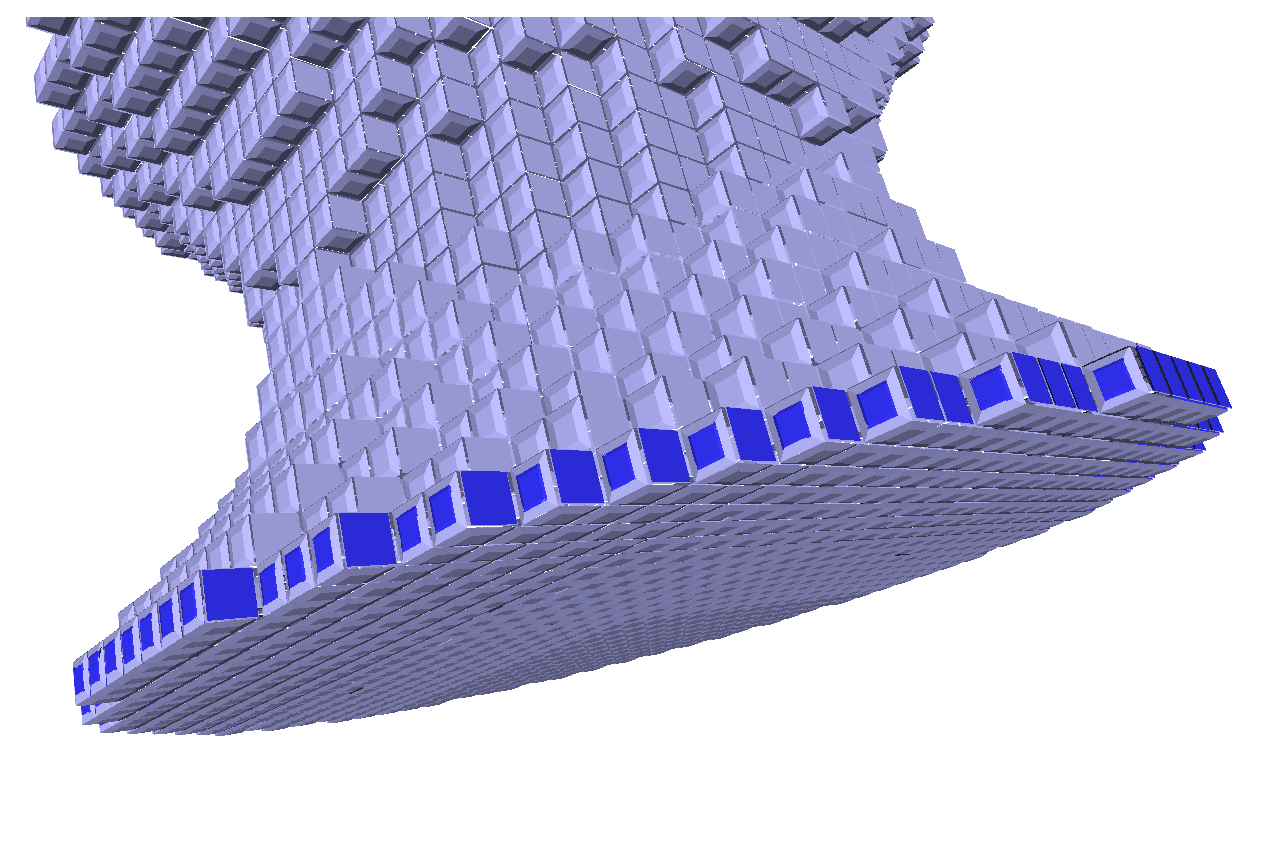
\includegraphics[width=0.3\textwidth]{gridCurve3d2}} 
\end{figure}
\end{frame}

\begin{frame}
  \frametitle{GridCurve}

  \begin{block}{Ranges}
GridCurve provides many ranges as nested types to iterate over different kinds of elements:
\begin{itemize}
   \item<1> SCellsRange: signed $d$-cells ($d \in \{1,(n-1)\}$)
   \item<2> PointsRange: digital coordinates of $0$-cells ($d \in \{1,(n-1)\}$)
   \item<3> MidPointsRange: real coordinates of $d$-cells ($d \in \{1,(n-1)\}$)
   \item<4> ArrowsRange: arrow coding of a signed $1$-cell ($d = 1$)
   \item<5> InnerPointsRange: digital coordinates of $n$-cells ($d = (n-1)$)
   \item<6> OuterPointsRange: digital coordinates of $n$-cells ($d = (n-1)$)
   \item<7> IncidentPointsRange: pair of inner and outer points
   \item<8> CodesRange (only for $n = 2$ and $d = 1$)
\end{itemize}
  \end{block}

\only<1>{
 \begin{center}
   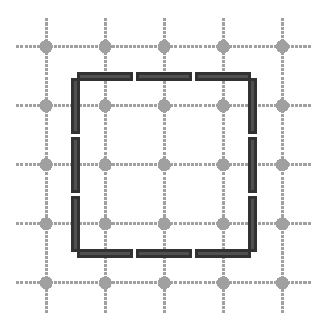
\includegraphics[height=0.25\textheight]{1cellsRange}
 \end{center}
}
\only<2>{
 \begin{center}
   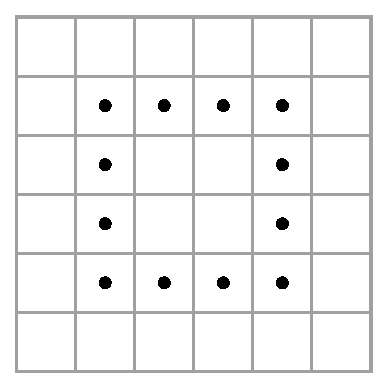
\includegraphics[height=0.25\textheight]{PointsRange}
 \end{center}
}
\only<3>{
 \begin{center}
   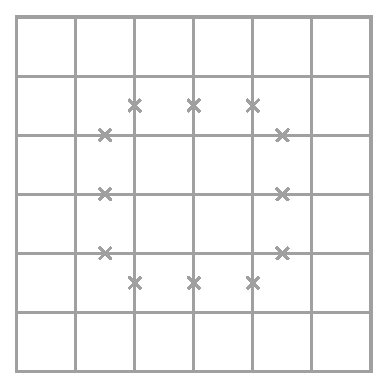
\includegraphics[height=0.25\textheight]{MidPointsRange}
 \end{center}
}
\only<4>{
 \begin{center}
   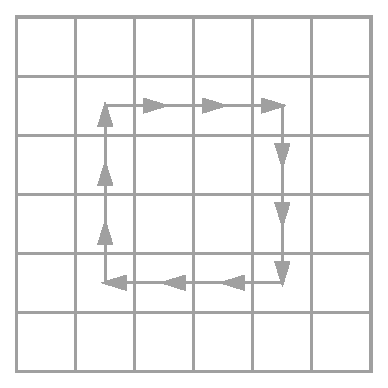
\includegraphics[height=0.25\textheight]{ArrowsRange}
 \end{center}
}
\only<5>{
 \begin{center}
   \includegraphics[height=0.25\textheight]{InnerPointsRange}
 \end{center}
}
\only<6>{
 \begin{center}
   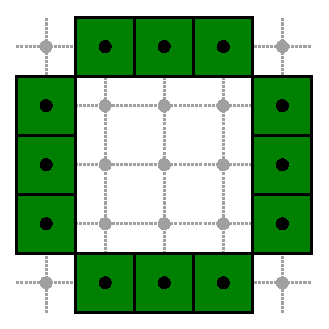
\includegraphics[height=0.25\textheight]{OuterPointsRange}
 \end{center}
}
\only<7>{
 \begin{center}
   \includegraphics[height=0.25\textheight]{IncidentPointsRange}
 \end{center}
}
\only<8>{
 \parbox[c][0.3\textheight]{1\textwidth}{ \begin{center} 1110002223333 \end{center} }
}
\end{frame}

%construction/initialisation ?

\begin{frame}[containsverbatim]
  \frametitle{GridCurve construction}

  \begin{lstlisting}
using namespace Z2i; //or Z3i
//cellular space
KSpace space;                 
//space bounds
space.init( Point::diagonal(0), Point::diagonal(50) );
//grid curve 
GridCurve<KSpace> gc(space); 
  \end{lstlisting}
... or easier in 2d (default dimension, coordinate type, space bounds): 
  \begin{lstlisting}
GridCurve<> gc; 
  \end{lstlisting}

\end{frame}


\begin{frame}[containsverbatim]
  \frametitle{GridCurve preparation}

GridCurve is empty after construction: 
  \begin{lstlisting}
ASSERT( gc.size() == 0 ); 
  \end{lstlisting}

Initialization from signed cells... 
  \begin{lstlisting}
gc.initFromSCellsRange( sCellsList.begin(), sCellsList.end() ); 
  \end{lstlisting}

... or initialization from points ($0$-cells in digital coordinates)
  \begin{lstlisting}
gc.initFromPointsRange( pointsList.begin(), pointsList.end() ); 
  \end{lstlisting}

Choosing its range: skeleton 
  \begin{lstlisting}
//typedef GridCurve::XXXRange Range; 
//Range r = gc.getXXXRange();
  \end{lstlisting}


\end{frame}

\begin{frame}[containsverbatim]
  \frametitle{GridCurve basic usage}

  \begin{lstlisting}
//choose a range
typedef GridCurve::CodesRange Range; 
Range r = gc.getCodesRange();
//do something 
if ( gc.isOpen() ) 
  doSomething( r.begin(), r.end() ); 
else 
  doSomething( r.c(), r.c() ); 
  \end{lstlisting}

  \begin{lstlisting}
template <typename CI>
void doSomething( const CI& ciBegin, const CI& ciEnd ) 
{
  BOOST_CONCEPT_ASSERT(( boost::BidirectionalIterator<CI> ));
  if ( isNotEmpty(ciBegin, ciEnd) ) 
  { //if the range is not empty
    CI i( ciBegin); 
    do 
    {
      ...
      i++;
    } while (i != ciEnd);
  }    
}
  \end{lstlisting}


\end{frame}

\begin{frame}
  \frametitle{GridCurve snapshot}

%graph
   \includegraphics[width=1\textwidth]{gridcurveGraph}

\end{frame}

